% Created 2024-04-25 Thu 01:14
% Intended LaTeX compiler: pdflatex
\documentclass[11pt]{article}
\usepackage[utf8]{inputenc}
\usepackage[T1]{fontenc}
\usepackage{graphicx}
\usepackage{longtable}
\usepackage{wrapfig}
\usepackage{rotating}
\usepackage[normalem]{ulem}
\usepackage{amsmath}
\usepackage{amssymb}
\usepackage{capt-of}
\usepackage{hyperref}
\usepackage{setspace}
\usepackage[gen]{eurosym}
\usepackage[labelfont=bf]{caption}
\doublespacing
\author{Hankertrix}
\date{\today}
\title{Will protecting right to repair mitigate the effects of climate change?}
\hypersetup{
 pdfauthor={Hankertrix},
 pdftitle={Will protecting right to repair mitigate the effects of climate change?},
 pdfkeywords={},
 pdfsubject={},
 pdfcreator={Emacs 29.3 (Org mode 9.6.15)}, 
 pdflang={English}}
\makeatletter
\newcommand{\citeprocitem}[2]{\hyper@linkstart{cite}{citeproc_bib_item_#1}#2\hyper@linkend}
\makeatother

\usepackage[notquote]{hanging}
\begin{document}

\maketitle
\setcounter{tocdepth}{2}
\tableofcontents \clearpage
\section{Introduction}
\label{sec:org7ffc864}
With the negative impact of climate change on human life growing in severity, it is crucial to implement mitigations to slow down or even stop climate change from progressing in severity, as well as adaptations to live with the current and future impacts of climate change. As such, this paper will focus on how protecting the right to repair will mitigate the effects of climate change.

\subsection{Right to repair}
\label{sec:org91bf852}
Right to repair is a legal right for owners of a piece of equipment, such as a vehicle or an electronic device, should be allowed to freely upgrade, modify or repair it (\citeprocitem{9}{Gisonna, 2023}; \citeprocitem{26}{Wikipedia, 2024}), which everyone already has. As such, the right to repair discussed in this paper is the effective right to repair, which refers to the ease and viability of repair by an owner of a piece of equipment. This effective right to repair has been eroded by manufacturers intentionally designing products to be difficult to repair (\citeprocitem{13}{Jefferys, 2021}; \citeprocitem{23}{Rossmann, 2018}), reducing the availability and accessibility of individual spare parts and diagnostic and calibration tools (\citeprocitem{14}{Jefferys, 2022}; \citeprocitem{24}{Rossmann, 2023}), and prohibiting independent repair providers from advertising on their platforms (\citeprocitem{10}{Google, n.d.}).

 \newpage

\subsubsection{Right to repair and climate change}
\label{sec:org12238e4}
The right to repair is closely intertwined with the concept of a circular economy (CE). In the circular economy, products are reused, repaired, refurbished and recycled to maximise the lifetime of the product. It also means minimising waste, as when products reach the end of their lifecycle, the materials from the product are not wasted and are instead fed back into the economy as spare parts or as recycled raw materials to repair or create new products (\citeprocitem{12}{Iacovidou et al., 2021}; \citeprocitem{16}{Kirchherr et al., 2017}; \citeprocitem{20}{Parliament, 2023}). The right to repair could result in a mindset shift away from consumerism, and towards an attitude of conservation and preservation of existing products, which is particularly important in the current consumerist world. This shift in attitude towards conservation would reduce the consumption and production of goods, which would also reduce the amount of greenhouse gases produced, mitigating the impacts of climate change. Improving the right to repair will also directly reduce the consumption and production of goods, as consumers will be more likely to buy more repairable products that will last for a long time, instead of short-lived products that need to be replaced quickly. As a result, manufacturers will also reduce the production of goods since consumers aren't purchasing as many products as before. Furthermore, since consumers can repair their devices for a much lower cost as compared to buying new products, they are more likely to repair their devices instead of throwing them away and buying a new product, which would result in less greenhouse gas emissions and hence mitigating the effects of climate change.


\section{Methodology}
\label{sec:orgab6cc99}

\subsection{France's repairability index}
\label{sec:org10da362}
France has implemented the repairability index to improve information regarding the feasibility of repair (\citeprocitem{8}{French Government, 2023}; \citeprocitem{22}{“Repairability index,” 2023}). It is a mandatory label that manufacturers must add to their electrical and electronic equipment to inform consumers of its repairability \textbf{(Figure \ref{fig:org1faf0ee})}. It covers 9 product categories, namely, computers, TVs, smartphones, lawnmowers, washing machines of all types, dishwashers, vacuum cleaners and high-pressure cleaners.

 \newpage

 \noindent The repairability index ranges from 0 to 10, and is calculated based on the following dimensions:
\begin{enumerate}
\item Documentation, which measures the number of years the manufacturer is committed to making technical documents freely available to repairers and consumers.
\item Disassembly and tools, which measures the ease of disassembly of the product. It depends on the type of tools required and the characteristics of the fasteners.
\item Spare parts, which measures the manufacturer's commitment to provide spare parts promptly.
\item Pricing, which measures the ratio between the price of spare parts and the price of the product.
\item Specific aspects, which is a sub-criteria specific to each product category.
\end{enumerate}

 \noindent An example of how the repairability index is calculated is shown in \textbf{Figure \ref{fig:org6c2a235}}.

 \newpage

\begin{figure}[!htbp]
\centering
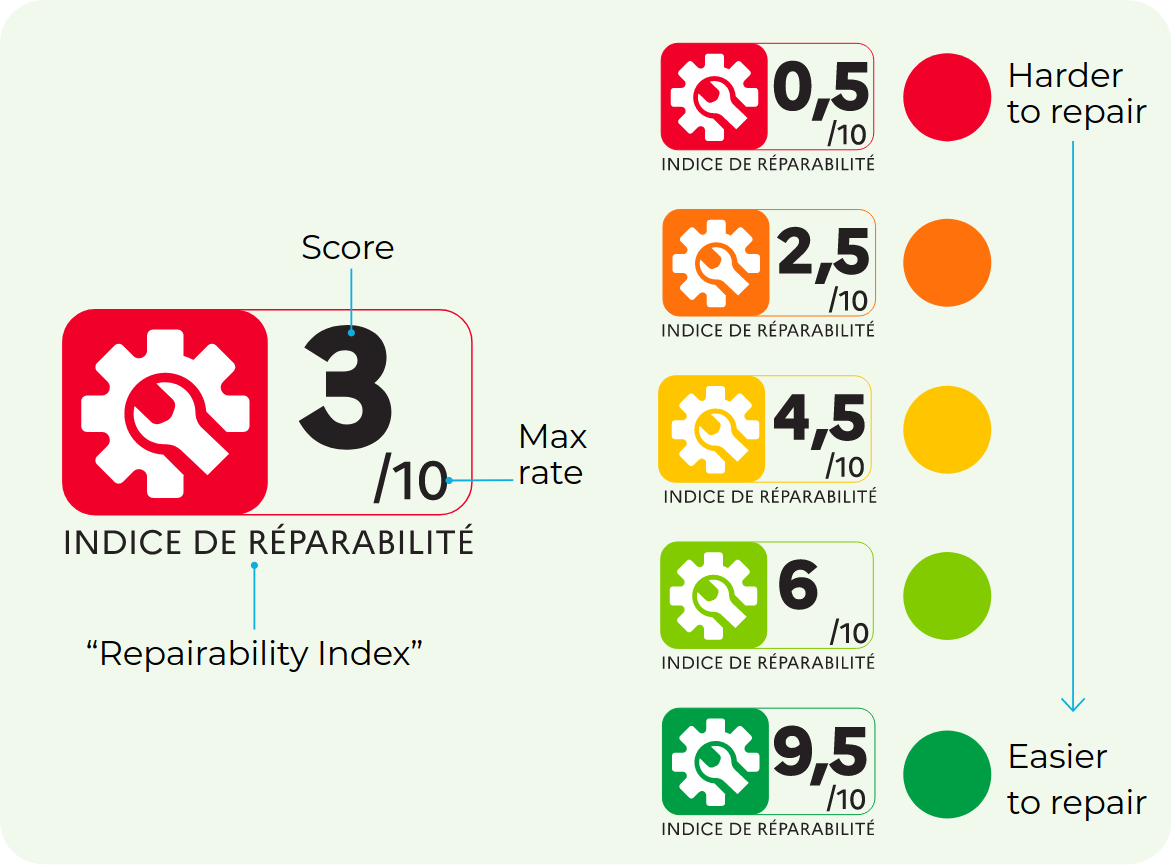
\includegraphics[scale=0.48]{./research-paper-images/repairability-index.png}
\caption{\label{fig:org1faf0ee}The repairability index label is mandatory to be displayed near the point of sale or provided upon request in France (\citeprocitem{22}{“Repairability index,” 2023}).}
\end{figure}

\begin{figure}[!htbp]
\centering
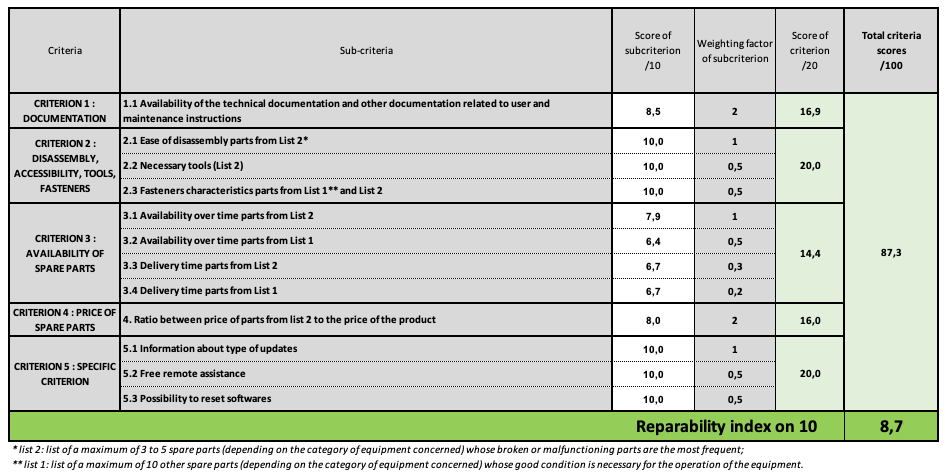
\includegraphics[scale=0.45]{./research-paper-images/fairphone-repairability-index.png}
\caption{\label{fig:org6c2a235}A scoresheet showing how the repairability index is calculated for the Fairphone 3+ (\citeprocitem{18}{Mdepypere, 2023}).}
\end{figure}

 \newpage

 \noindent The repairability index for every product is self-reported by the manufacturer, which is computed by having the manufacturers enter the required parameters into a spreadsheet which then computes the index (\citeprocitem{18}{Mdepypere, 2023}). The manufacturer must also provide the scoresheet within 15 days upon request from the consumer. The French government will also fine any manufacturer that has been found falsifying the repairability index.

\subsection{Legislation against planned obsolescence in France}
\label{sec:orge7da534}
France revised its consumer code in 2015 and became the first country to ban planned obsolescence (\citeprocitem{17}{Maitre-Ekern \& Dalhammar, 2016}). Planned obsolescence refers to the techniques employed by manufacturers that aim to deliberately reduce the lifespan of a product to increase the rate of replacement of a product. Manufacturers who engage in planned obsolescence are punished with 2 years of imprisonment and a fine of \(\euro{300,000}\) (\citeprocitem{2}{Bates-Prince, 2018}). This law aims to reduce the amount of e-waste generated by manufacturers using planned obsolescence to force consumers to throw away perfectly usable products. In 2017, an activist by the name of Laetitia Vasseur filed a lawsuit against Apple for intentionally slowing down old iPhones through software updates to get customers to replace them (\citeprocitem{19}{Miazaki, 2024}). Apple famously claimed that it slowed down older iPhone models to preserve the battery life, but they still ended up being fined \(\euro{25}\) million by the French government for slowing down older iPhones (\citeprocitem{4}{BBC, 2020}; \citeprocitem{7}{Dillet, 2020}; \citeprocitem{15}{Kayali, 2020}; \citeprocitem{21}{Porter, 2020}; \citeprocitem{25}{Sonnemaker, 2020}).

\section{Results}
\label{sec:org971d029}

\subsection{France's repairability index}
\label{sec:org111a00b}
The policy has been effective in changing consumer behaviour, as 76\% of consumers now take into account the repairability index when making a purchasing decision (\citeprocitem{11}{HOP, 2022}). This result shows the importance of making repairability information clear and easily accessible to consumers, as it can do a lot to change consumer behaviour. It also shows that consumers in France are willing to buy products that are more repairable and hence more environmentally friendly. This mindset can also be seen in other countries, especially for consumers in India, Indonesia, Poland and the United Arab Emirates (UAE) (\citeprocitem{5}{Bruce, 2021}). The index also coerces manufacturers to make their products more repairable, as having a repairability index of 6 is a nice green colour, which is far more appealing to consumers than the red, orange and yellow colours of the lower indexes (\textbf{Figure \ref{fig:org1faf0ee}}).

 \newpage

 \noindent However, since manufacturers are responsible for their repairability index and there is no external verification in the process, the repairability index could be inflated. While blatant falsification could result in hefty fines for manufacturers, manufacturers can improve their repairability index by a decent amount by improving their scores for certain categories. Stop Planned Obsolescence (HOP) found that quite a few products had inflated repairability indexes, like the Apple MacBook Pro, the Apple iPhone 7+, the Samsung Galaxy A41 and the Vivo Y21s (\citeprocitem{11}{HOP, 2022}). These were mostly due to different interpretations of the criteria by HOP and the manufacturers, of which the manufacturers were more likely to interpret the criteria in ways that would inflate their repairability index.

 \noindent Furthermore, certain criteria can be considered as key for repairability, such as disassembly. For example, a product that is glued or welded is inherently difficult to disassemble and is hence difficult, or even impossible to repair in the latter case. However, since the different criteria have nearly equal weightage, a manufacturer can simply provide easy access to documentation and repair manuals to raise their repairability index by a significant amount, despite not making the product significantly more repairable due to the difficulty in disassembly.

 \newpage

 \noindent As such, more stringent definitions are needed and the criteria will need to be refined to make sure that the repairability index is an accurate indicator of the repairability of a product. Without these changes, consumers may lose trust in the repairability index, which would render the index useless. Consumers may also deflate the repairability scores, seeing as so many manufacturers have overinflated repairability scores, which would result in truly repairable products being dismissed by consumers as they are rated similarly to less repairable products.

\subsection{Legislation against planned obsolescence in France}
\label{sec:org2d44e6f}
As a result of the legislation against planned obsolescence, Apple provided large discounts for battery replacements for the affected devices, which stopped the throttling of the devices (\citeprocitem{3}{BBC, 2018}). This move encouraged consumers to replace the batteries in their older devices instead of buying a new device, which ultimately reduced e-waste. Furthermore, this legislation provided a platform for activists to pursue legal action against companies that engaged in planned obsolescence, such as the printer company Epson. Therefore, this legislation will likely force manufacturers to stop using planned obsolescence as a way to earn more revenue from their customers, for fear of massive fines as a result of legal action from the government, consumers and activists. It also allows the government to punish companies for planned obsolescence directly, instead of using related laws, which may be more difficult to enforce and exact punishments.

 \newpage

 \noindent However, it can be difficult to prove the manufacturer's intent, as the law states that the reduction in the lifespan of a product must be deliberate, which can be very difficult to prove as the manufacturers can come up with a vast number of different excuses and reasons to make their actions accidental rather than intentional. Therefore, more specific guidelines and regulations can be put in place, in addition to this law, to make it easier to convict and punish manufacturers for engaging in planned obsolescence instead of trying to prove their malicious intent, which is rather difficult to do.

 \newpage

\section{Discussion}
\label{sec:org6da0dba}

\subsection{France's repairability index}
\label{sec:org6f6c722}

\subsubsection{Feasibility}
\label{sec:orgc454f89}
The repairability index should be relatively practical to implement in most developed countries, as France has already laid the groundwork for similar laws to build upon. It will most probably also result in consumers being conscious about the repairability of products and hence choosing to purchase repairable products as a majority of consumers strive to be environmentally friendly (\citeprocitem{1}{Am et al., 2023}). However, for developing countries, such legislation may not be very useful as such countries have other more pressing problems that they have to deal with.

\subsubsection{Improvements}
\label{sec:orgfc79074}
There are some shortcomings in France's implementation of the repairability index that will need to be addressed. The first is to have more stringent and clearer definitions of the various categories and how they are accessed, so that the self-reported repairability scores by manufacturers are accurate. This will also allow for third-party validation of the repairability index to be more consistent, which builds consumer trust in the repairability index.

 \newpage

 \noindent Secondly, having the repairability index self-reported by the manufacturers is not ideal. It would be much better to have a governmental regulatory agency that verifies the repairability scores submitted by manufacturers, which will improve the accuracy of the repairability index. However, this may increase the costs of implementing such an index. Despite this, the regulatory agency also allows the government to force manufacturers to provide information to the regulatory agency for verification, which solves the problem of third-party organisations not being able to obtain information from manufacturers, such as the prices of spare parts from Apple, due to the repair shops being in non-disclosure agreements (NDAs) with Apple (\citeprocitem{11}{HOP, 2022}). Also, to discourage manufacturers from overinflating their repairability scores, punishments such as fines can be implemented if the repairability index from the manufacturer deviates by a certain amount or more from the repairability index from the regulatory agency, like 0.5 points or something similar. Additionally, it may be beneficial to have legislation forcing manufacturers to disclose information that is required for a third party to independently evaluate a product's repairability index. This way, manufacturers are unable to inflate a product's repairability index without public backlash and are also unable to overcharge consumers for repair, which would result in more consumers choosing to repair their devices as repair is cheaper, reducing e-waste and greenhouse gas emissions, mitigating the effects of climate change.

 \newpage

 \noindent Lastly, the repairability index needs to have the weightage adjusted for different categories as some categories are far more important to repairability than others. For example, the ease of disassembly and the cost and availability of spare parts are more important to repairability compared to documentation. Changing the weightage of the categories in line with their importance regarding repairability would make the repairability index more representative of the product's actual repairability and increase consumer trust in the repairability index. This way, manufacturers cannot inflate their repairability index by providing more documentation, which forces them to make products that are easier to disassemble and use standard parts to get a decent repairability index. This would ultimately reduce the cost of repair for consumers, which will result in more consumers choosing to repair rather than replace their products, reducing the amount of e-waste generated.

 \noindent Another way to address this issue is to have the scores in certain categories that are easy to achieve be capped at a certain amount if the scores in the other categories have not reached a certain threshold. For example, the scores for documentation can be capped at 5 if the score for disassembly and spare parts is lower than 10. This would allow the weightage for each of the categories to be equal but still achieve the same effect. This could also be easier to refine and tweak compared to a weight. However, this approach would make understanding the law more difficult as the calculation of the repairability index is now more convoluted which can result in more confusion for both manufacturers and consumers.

 \newpage

 \noindent With all these changes, it could make the repairability index much more difficult and costly to implement, but it would result in an index that is more representative of the repairability of a product which would coerce manufacturers to make more repairable products. Since consumers are generally environmentally conscious and want to be environmentally friendly (\citeprocitem{1}{Am et al., 2023}), this will result in an eventual shift to more repairable products. With consumers having products that have a longer lifespan and a longer support period, they'll replace their products less often and hence less e-waste and greenhouse gases are produced. This could also result in manufacturers reducing the amount of products produced and having fewer product releases, which will also reduce the amount of e-waste and greenhouse gas generated.

 \newpage

\subsection{Legislation against planned obsolescence}
\label{sec:org05586eb}

\subsubsection{Feasibility}
\label{sec:orgeef4145}
Legislation banning planned obsolescence should be trivial to pass in pretty much every single country, as the law in itself is very simple. However, to ensure that the law is being enforced and that manufacturers are not engaging in planned obsolescence, it will require a lot of resources to investigate and prove the manufacturer's malicious intentions. This can make enforcement difficult, as big manufacturers such as Apple, Google and Samsung can hire excellent lawyers that can prove otherwise (\citeprocitem{6}{“Companiesmarketcap.com - companies ranked by market capitalization,” 2024}), which would make legal battles extremely expensive as they will drag out over a long time and may end up with no result, costing the government a lot of money in the process. Despite this, having such a law will give the government the ability to convict manufacturers for engaging in planned obsolescence without needing to use another, less directly applicable law to convict them, making it easier to convict manufacturers who are engaging in the practice.

 \newpage

\subsubsection{Improvements}
\label{sec:org4a396ef}
A law that bans planned obsolescence will need to be supported with other laws such as minimum lifetime guarantees or design requirements to make it easier to convict manufacturers who engage in planned obsolescence, as such laws are well-defined and have a set standard for manufacturers to meet, which makes it very clear if manufacturers are breaking the law. However, these changes will ultimately increase the cost of enforcement as the government will need to set up or employ an agency to handle the auditing of companies to ensure that they comply with the laws. This may cost even more than the cost of a long, drawn-out legal battle between the government and a big manufacturer, as this enforcement will apply to all manufacturers. However, these improvements are not strictly necessary and can be omitted in developing countries where the government doesn't have the budget to enforce these laws. Having a ban on planned obsolescence could be sufficient to dissuade manufacturers from engaging in the practice if it is well-enforced.

 \newpage

\section{Conclusion}
\label{sec:org608e3e5}
With the right to repair directly affecting the production and consumption of goods, implementing legislation to protect the right to repair will likely mitigate the effects of climate change. Furthermore, protecting and improving the consumer's right to repair will most likely result in a mindset shift away from consumerism and towards repairability, quality and conservation. Due to having a greater right to repair, consumers will most likely find repairing products to be far more economically viable compared to replacing their products, which will cause them to prefer repairable products to cheap products, as it will save them more money, as well as time when migrating their data over to the new product in the long term. This is seen in the results section, where the repairability index has caused 76\% of consumers to consider repairability when making purchasing decisions. Even though the index doesn't directly improve the consumers' right to repair, as it only makes it much easier for consumers to gauge the repairability of a product at a glance, it still greatly influences consumer behaviour. Improving the consumers' right to repair would likely result in larger changes in consumer behaviour towards conservation and sustainability. Likewise, producers would adapt to this shift in consumer behaviour and make products that are of higher quality and are more repairable to appeal to consumers, which will reduce the number of goods produced, reducing the amount of waste and greenhouse gas emissions produced and mitigating the effects of climate change.

 \newpage

\section{References}
\label{sec:orgf00369a}
\begin{hangparas}{1.5em}{1}
\hypertarget{citeproc_bib_item_1}{Am, J. B., Doshi, V., Noble, S., \& Malik, A. (2023, February). Consumers care about sustainability-and back it up with their wallets. \textit{Mckinsey \& Company}. McKinsey \& Company. Retrieved from \url{https://www.mckinsey.com/industries/consumer-packaged-goods/our-insights/consumers-care-about-sustainability-and-back-it-up-with-their-wallets}}

\hypertarget{citeproc_bib_item_2}{Bates-Prince, J. (2018, May). Interview: The story of france’s fight against planned obsolescence. \textit{Buy Me Once}. Retrieved from \url{https://buymeonce.com/blogs/articles-tips/interview-france-fight-planned-obsolescence}}

\hypertarget{citeproc_bib_item_3}{BBC, N. (2018, January). Apple investigated by france for “planned obsolescence”. \textit{Bbc News}. BBC. Retrieved from \url{https://www.bbc.com/news/world-europe-42615378}}

\hypertarget{citeproc_bib_item_4}{BBC, N. (2020, February). Apple fined for slowing down old iphones. \textit{Bbc News}. BBC. Retrieved from \url{https://www.bbc.com/news/technology-51413724}}

\hypertarget{citeproc_bib_item_5}{Bruce, G. (2021, February). Global data: Most consumers would prefer to repair broken tech, rather than replace it. \textit{Yougov}. YouGov. Retrieved from \url{https://today.yougov.com/technology/articles/34350-repair-replace-tech-global-data}}

\hypertarget{citeproc_bib_item_6}{Companiesmarketcap.com - companies ranked by market capitalization. (2024, April). \textit{Companiesmarketcap.Com - Companies Ranked by Market Capitalization}. Retrieved from \url{https://companiesmarketcap.com/}}

\hypertarget{citeproc_bib_item_7}{Dillet, R. (2020, February). Apple fined \$27 million in france for throttling old iphones without telling users. \textit{Techcrunch}. TechCrunch. Retrieved from \url{https://techcrunch.com/2020/02/07/apple-fined-27-million-for-throttling-old-iphones-without-telling-users/}}

\hypertarget{citeproc_bib_item_8}{French Government, F. (2023, December). Indice de réparabilité. \textit{Ministère de La Transition Écologique et de La Cohésion Des Territoires}. French Government. Retrieved from \url{https://www.ecologie.gouv.fr/indice-reparabilite}}

\hypertarget{citeproc_bib_item_9}{Gisonna, N. (2023). Right to repair. In \textit{Encyclopedia britannica}. Retrieved from \url{https://www.britannica.com/topic/right-to-repair}}

\hypertarget{citeproc_bib_item_10}{Google. (n.d.). Advertising policies help, other restricted businesses: Third-party consumer technical supporturlhttps://support.google.com/adspolicy/answer/13527027. \textit{Google}. Google.}

\hypertarget{citeproc_bib_item_11}{HOP. (2022, February). The french repairability index: A first assessment – one year after its implementation. \textit{Stop to Planned Obsolescence}. Retrieved from \url{https://www.halteobsolescence.org/wp-content/uploads/2022/02/Rapport-indice-de-reparabilite.pdf}}

\hypertarget{citeproc_bib_item_12}{Iacovidou, E., Hahladakis, J. N., \& Purnell, P. (2021). A systems thinking approach to understanding the challenges of achieving the circular economy. \textit{Environmental Science and Pollution Research}, \textit{28}, 24785–24806.}

\hypertarget{citeproc_bib_item_13}{Jefferys, H. (2021, January). Samsung starts blocking 3rd party repairs? - galaxy a51 teardown and repair assessment. \textit{Youtube}. YouTube. Retrieved from \url{https://www.youtube.com/watch?v=zGLQ9ZRntZo}}

\hypertarget{citeproc_bib_item_14}{Jefferys, H. (2022, May). Apples self repair program is not what it seems. \textit{Youtube}. YouTube. Retrieved from \url{https://www.youtube.com/watch?v=SQbVuhwwd4s}}

\hypertarget{citeproc_bib_item_15}{Kayali, L. (2020, February). Apple fined €25m in france for misleading consumers about slowed-down iphones. \textit{Politico}. POLITICO. Retrieved from \url{https://www.politico.eu/article/apple-fined-e25m-in-france-for-misleading-consumers-about-slowed-down-iphones/}}

\hypertarget{citeproc_bib_item_16}{Kirchherr, J., Reike, D., \& Hekkert, M. (2017). Conceptualizing the circular economy: An analysis of 114 definitions. \textit{Resources, Conservation and Recycling}, \textit{127}, 221–232.}

\hypertarget{citeproc_bib_item_17}{Maitre-Ekern, E., \& Dalhammar, C. (2016). Regulating planned obsolescence: a review of legal approaches to increase product durability and reparability in europe. \textit{Review of European, Comparative \& International Environmental Law}, \textit{25}(3), 378–394.}

\hypertarget{citeproc_bib_item_18}{Mdepypere. (2023, February). The french repair index: Challenges and opportunities. \textit{Right to Repair Europe}. Retrieved from \url{https://repair.eu/news/the-french-repair-index-challenges-and-opportunities/}}

\hypertarget{citeproc_bib_item_19}{Miazaki, V. (2024, March). Is france making planned obsolescence obsolete? \textit{Craftsmanship Magazine}. Craftsmanship Magazine. Retrieved from \url{https://craftsmanship.net/is-france-making-planned-obsolescence-obsolete/}}

\hypertarget{citeproc_bib_item_20}{Parliament, E. (2023, May). Circular economy: Definition, importance and benefits: Topics: European parliament. \textit{Topics | European Parliament}. European Parliament. Retrieved from \url{https://www.europarl.europa.eu/topics/en/article/20151201STO05603/circular-economy-definition-importance-and-benefits}}

\hypertarget{citeproc_bib_item_21}{Porter, J. (2020, February). Apple hit with €25 million fine in france for iphone slowdown controversy. \textit{The Verge}. The Verge. Retrieved from \url{https://www.theverge.com/2020/2/7/21127984/apple-iphone-batterygate-slowdown-batteries-french-fine}}

\hypertarget{citeproc_bib_item_22}{Repairability index. (2023, February). \textit{One Planet Network}. One Planet Network. Retrieved from \url{https://www.oneplanetnetwork.org/sites/default/files/from-crm/23_02_02_Case_Index.pdf}}

\hypertarget{citeproc_bib_item_23}{Rossmann, L. (2018, April). The horrible truth about apple’s repeated engineering failures. \textit{Youtube}. YouTube. Retrieved from \url{https://www.youtube.com/watch?v=AUaJ8pDlxi8}}

\hypertarget{citeproc_bib_item_24}{Rossmann, L. (2023, March). Apple withholds calibration tool for sleep sensors on modern macbooks from independent repair shops. \textit{Youtube}. YouTube. Retrieved from \url{https://www.youtube.com/watch?v=RIFQC8iA65k}}

\hypertarget{citeproc_bib_item_25}{Sonnemaker, T. (2020, February). France just fined apple \$27 million for intentionally slowing down iphones - the amount of profit the company makes in under 3 hours. \textit{Business Insider}. Business Insider. Retrieved from \url{https://www.businessinsider.com/france-fines-apple-27-million-for-intentional-iphone-throttling-2020-2}}

\hypertarget{citeproc_bib_item_26}{Wikipedia, W. F. (2024, March 7). Right to repair. Retrieved from \url{https://en.wikipedia.org/wiki/Right_to_repair}}\bigskip
\end{hangparas}

\[\text{Word count: 2911}\]
\[\text{Number of references: 26}\]
\end{document}
